\section{Architecture Integration}

\subsection{Model Support}

\begin{table}[H]
\centering
\small
\begin{tabular}{lllllll}
\toprule
\textbf{Model} & \textbf{Attention path} & \textbf{Nested?} & \textbf{RoPE?} & \textbf{GQA?} & \textbf{Relative?} & \textbf{Cross?} \\
\midrule
DistilBERT & \texttt{layer[i].attention} & No & No & No & No & No \\
RoBERTa & \texttt{layer[i].attention.self} & Yes & No & No & No & No \\
GPT-2 & \texttt{h[i].attn} & No & No & No & No & No \\
Qwen3.5 & \texttt{layers[i].self\_attn} & No & Yes & Yes & No & No \\
T5 & \texttt{block[i].layer[0].SelfAttention} & No & No & No & Yes & Yes (layer[1]) \\
\bottomrule
\end{tabular}
\end{table}

\subsection{Weight Extraction}

Our \texttt{copy\_weights} handles five patterns:

\subsubsection{UniversalAdapter First}

\begin{lstlisting}
from framework.core.adapters import UniversalAdapter
w, b = UniversalAdapter.get_weight_bias(src, proj)  # proj $\in$ {"q", "k", "v", "o"}
\end{lstlisting}

Handles most standard architectures.

\subsubsection{GPT-2 Conv1D}

\begin{lstlisting}
fused_w = src.c_attn.weight.T
fused_b = src.c_attn.bias
q_w, k_w, v_w = fused_w.chunk(3, dim=0)
\end{lstlisting}

\subsubsection{RoBERTa Nested}

\begin{lstlisting}
s = src.self
q_w = s.query.weight
k_w = s.key.weight
v_w = s.value.weight
o_w = src.output.dense.weight
\end{lstlisting}

\subsubsection{DistilBERT Flat}

\begin{lstlisting}
q_w = src.q_lin.weight
k_w = src.k_lin.weight
v_w = src.v_lin.weight
o_w = src.out_lin.weight
\end{lstlisting}

\subsubsection{Fallback `<proj>\_proj`}

\begin{lstlisting}
mod = getattr(src, f"{proj}_proj")
w = mod.weight
\end{lstlisting}

\subsection{Handling `W\_O` Factor}

Unlike SOA Fused Attention, we \textbf{do not skip $W_O$}. We apply the same 
factorization procedure, with the residual adapter absorbing approximation 
error.

For nested encoders, the outer \texttt{attention.output.dense} is \textbf{replaced} with 
our factorized \texttt{out\_proj}. The \texttt{is\_nested\_encoder} flag remains for the 
forward pass, but the output projection is applied inside our module.

\subsection{T5 Relative Bias Transfer}

\begin{lstlisting}
if hasattr(src, "relative_attention_bias") and src.relative_attention_bias is not None:
    self.relative_attention_bias = src.relative_attention_bias
    self.has_relative_attention_bias = True
\end{lstlisting}

In \texttt{compute\_bias}, we generate the position bias for any (query, key) pair.

\subsection{Cross-Attention}

The forward pass handles cross-attention by inspecting \texttt{key\_value\_states}:

\begin{lstlisting}
key_value_states = kwargs.get("key_value_states", encoder_hidden_states)
is_cross_attention = key_value_states is not None
kv_input = key_value_states if is_cross_attention else hidden_states
\end{lstlisting}

K, V are computed from \texttt{kv\_input}; Q from \texttt{hidden\_states}. The factorized 
projections apply identically.

\subsection{Causal Detection}

Robust prefix matching:

\begin{lstlisting}
_decoder_prefixes = ("gpt", "qwen", "llama", "mistral", "gemma", "phi",
                     "opt", "bloom", "falcon", "olmo", "mpt", "stablelm")
is_dec = any(model_type.startswith(p) for p in _decoder_prefixes)
\end{lstlisting}

Also checks \texttt{config.is\_decoder}, \texttt{config.is\_causal}, \texttt{config.causal}, and 
the source attention's attributes.

\subsection{Injection Algorithm}

\textbf{Algorithm 2:} Inject Adaptive SVD Attention into a model
\begin{lstlisting}
Input:  model M, config c, svd_rank, residual_rank, energy_threshold
Output: M with attention replaced

1: for each layer with attention:
2:     src $\leftarrow$ extract_attention(layer)
3:     if src is None or is_already_injected: continue
4:     try:
5:         new $\leftarrow$ AdaptiveSVDAttention(c, ..., pretrained_attn=src)
6:         replace(layer, new)
7:     except Exception as e:
8:         log_error(f"Layer failed: {e}")
9:         continue
10: return M
\end{lstlisting}

\subsection{Failure Handling}

Two-stage error handling:

\textbf{Stage 1 -- Pre-flight test:} Construct the module inside a try/except. If 
construction fails (weight extraction issue), return \texttt{None} and skip.

\textbf{Stage 2 -- Frobenius validation:} If construction succeeds but a 
projection has near-zero norm, raise \texttt{RuntimeError}.

\begin{lstlisting}
try:
    test_module = AdaptiveSVDAttention(..., pretrained_attn=old_attn)
except Exception:
    return None
\end{lstlisting}

\subsection{Registry}

\begin{lstlisting}
@ATTENTION_REGISTRY.register("adaptive_svd_attn")
@ATTENTION_REGISTRY.register("adaptive_svd")
@ATTENTION_REGISTRY.register("adaptive_svd_attention")
class AdaptiveSVDAttention(BaseAttention):
    ...
\end{lstlisting}

\subsection{Double-Injection Guard}

\begin{lstlisting}
if isinstance(src_attn, AdaptiveSVDAttention): return None
if "AdaptiveSVD" in src_attn.__class__.__name__: return None
\end{lstlisting}



\begin{figure}[H]
\centering
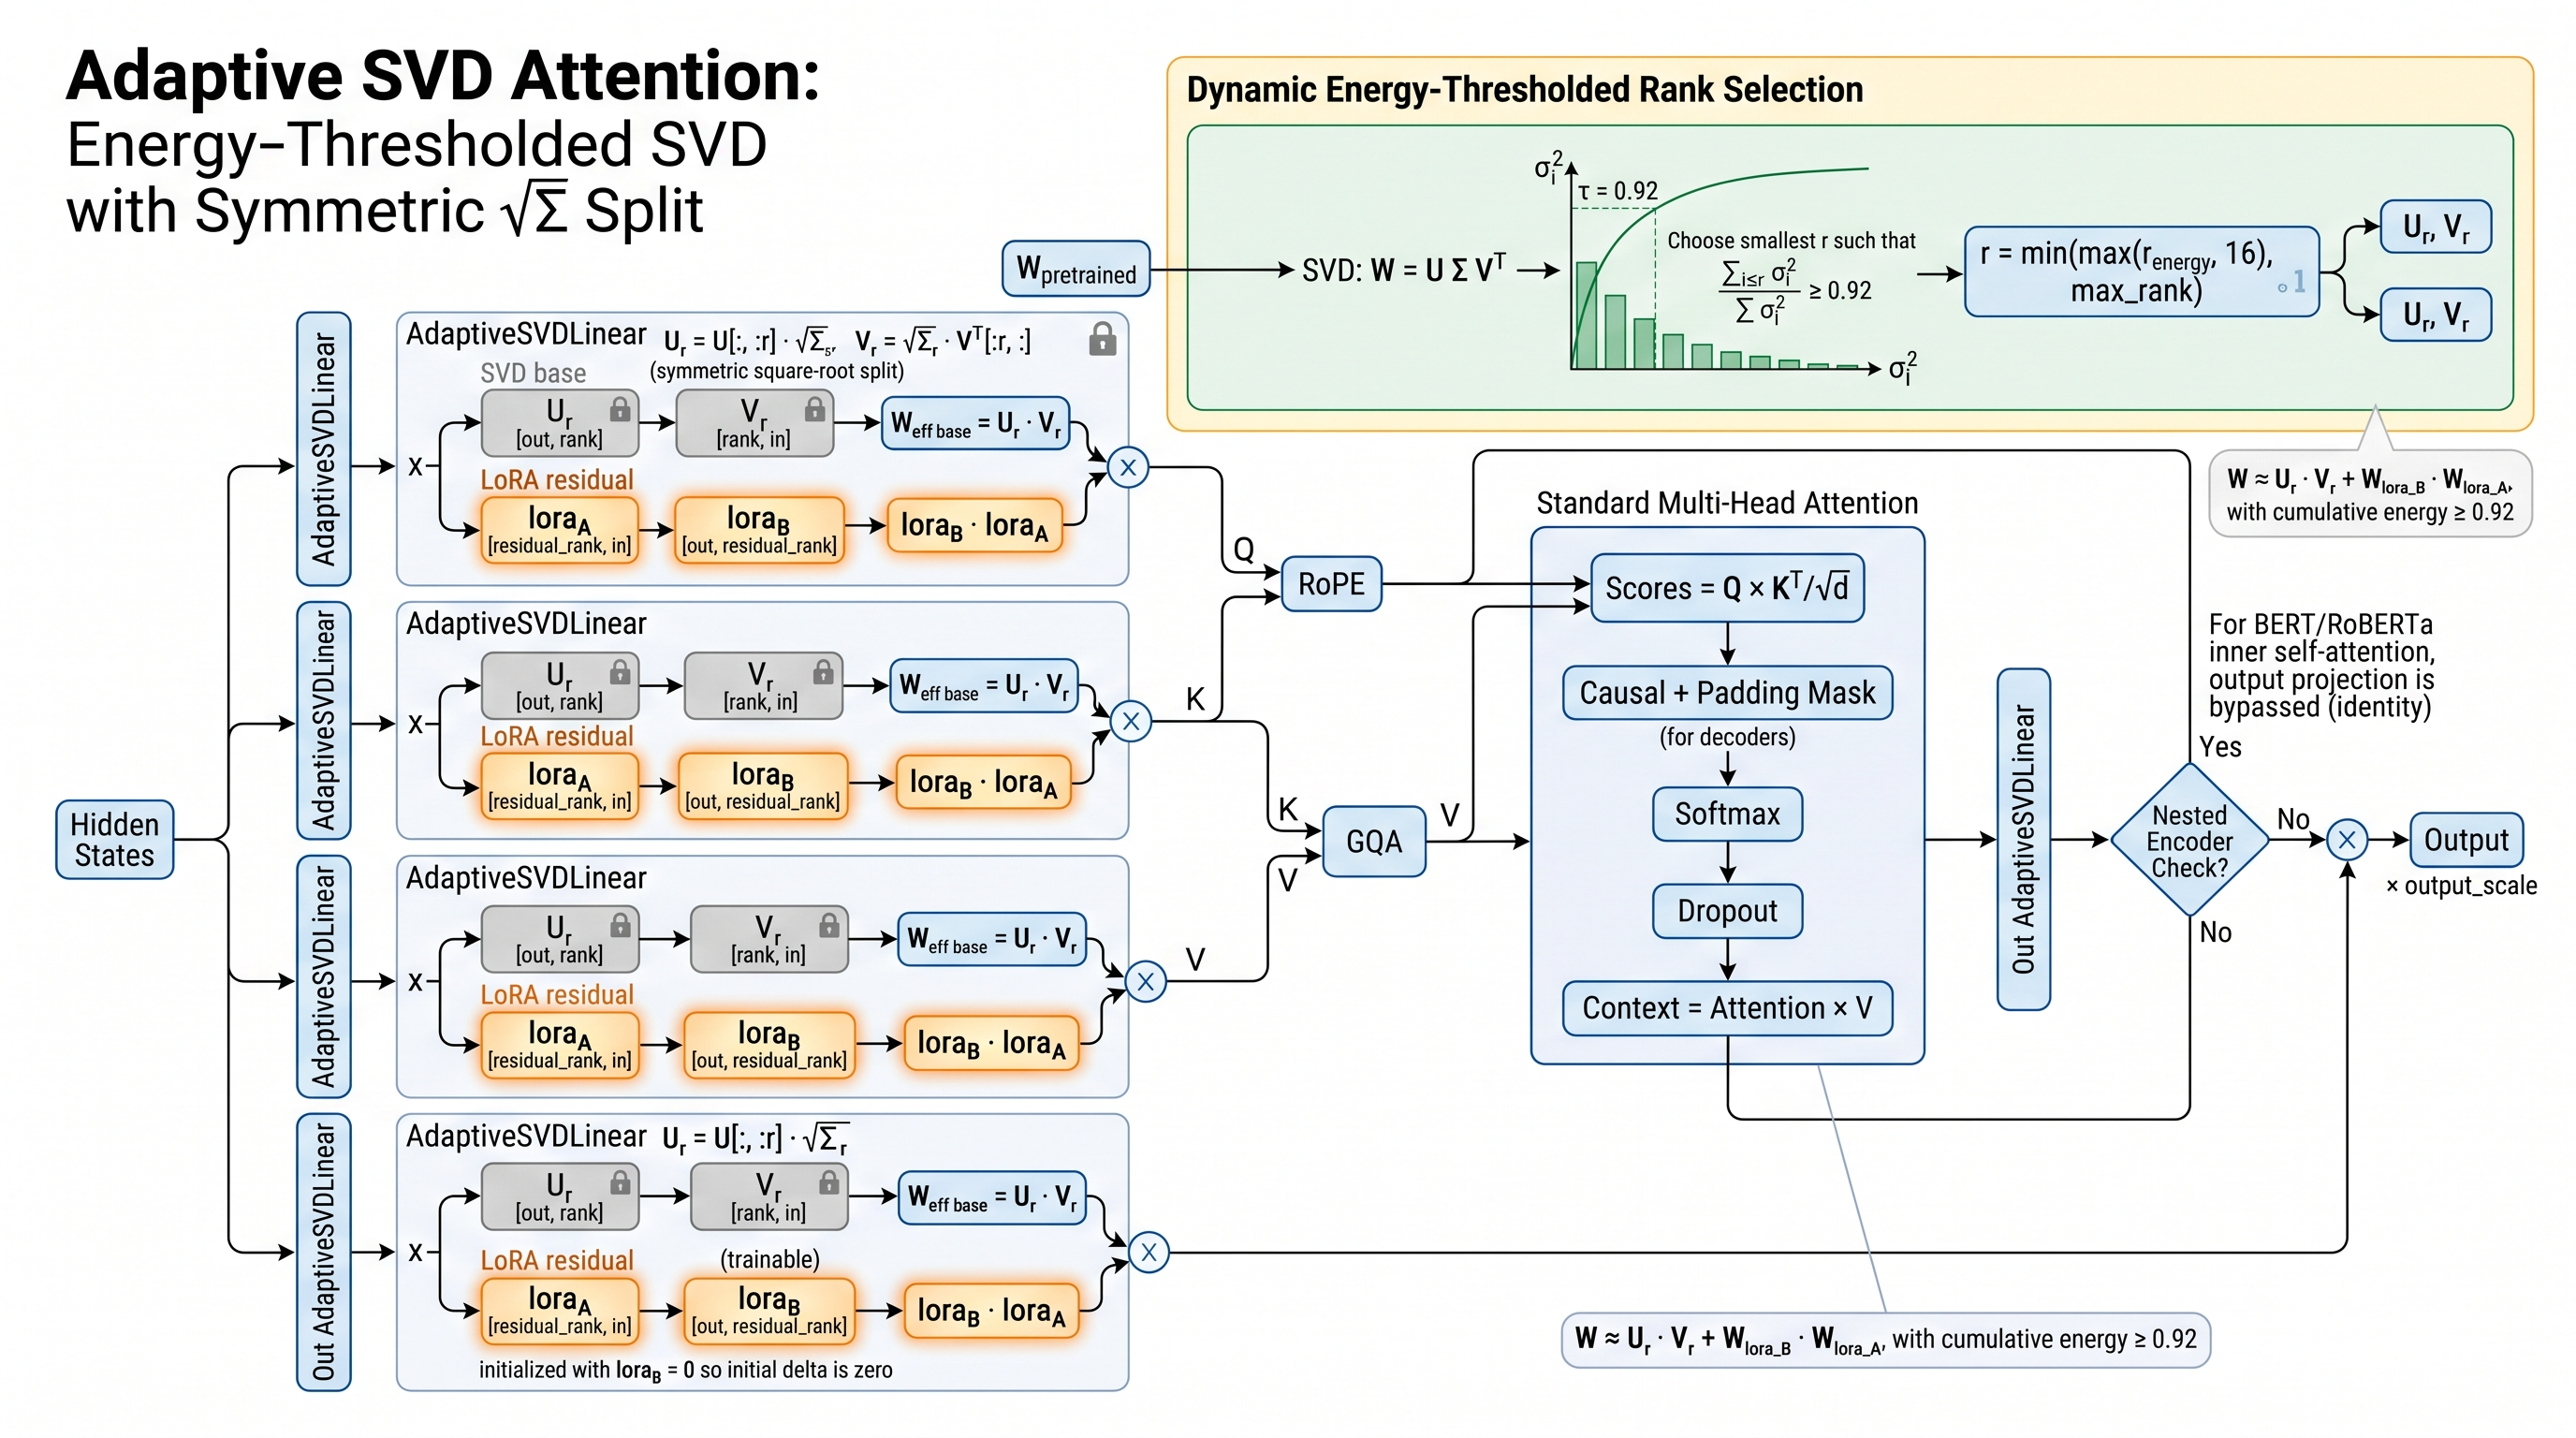
\includegraphics[width=\linewidth]{figures/architecture.jpeg}
\caption{High-level architectural diagram of adaptive\_svd\_attention.}
\label{fig:arch_adaptive-svd-attention}
\end{figure}

